\documentclass[tikz]{standalone}

\usetikzlibrary{shapes,arrows.meta,positioning}

\begin{document}
	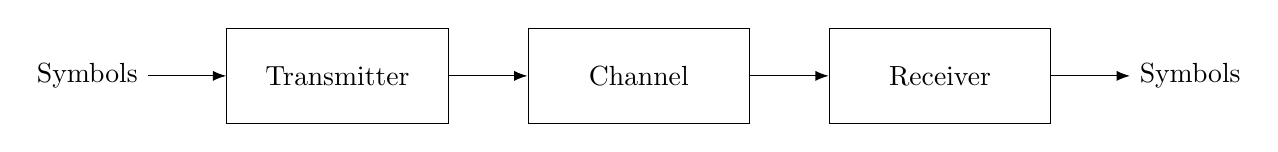
\begin{tikzpicture}[
		block/.style={draw, minimum height=8ex, minimum width=8em}
	]
		\node (sym in) {Symbols};
		\node[block, right=of sym in] (tx) {Transmitter};
		\node[block, right=of tx] (ch) {Channel};
		\node[block, right=of ch] (rx) {Receiver};
		\node[right=of rx] (sym out) {Symbols};

		\draw[-Latex] (sym in) -- (tx);
		\draw[-Latex] (tx) -- (ch);
		\draw[-Latex] (ch) -- (rx);
		\draw[-Latex] (rx) -- (sym out);
	\end{tikzpicture}
\end{document}